\chapter{[En curso] Marco teórico y contexto tecnológico}
\label{chapter:marco}

\chapquote{Una vez que algo es una pasión, hay motivación.}{Michael Schumacher}

\section{Marco Teórico}


%En este capítulo se introducen los conceptos teóricos sobre los que se asienta el desarrollo de este proyecto. Con el contenido de este capítulo se espera
%crear un base de conocimiento sobre la que desarrollar el resto de este documento. Además, se realiza un análisis de las herramientas que se van a emplear para desarrollar el sistema y cómo estas se encuadran en el contexto tecnológico actual.
%
%\section{Sistemas IoT}
%
%Tal y como se introdujo de manera informal en el capítulo anterior, \textit{IoT} se define como un sistema global e inteligente
%sistema con conciencia global, transmisión fiable
%y procesamiento inteligente de datos %\cite{noauthor_8_2020}.
%
%En este sentido una arquitectura de alto nivel, basada en el conjunto de capas de todos estos objetos interconectados puede verse representada gráficamente en la Figura \ref{fig:IoT_General}.
%
%\begin{figure}[H]
%  \centering
%  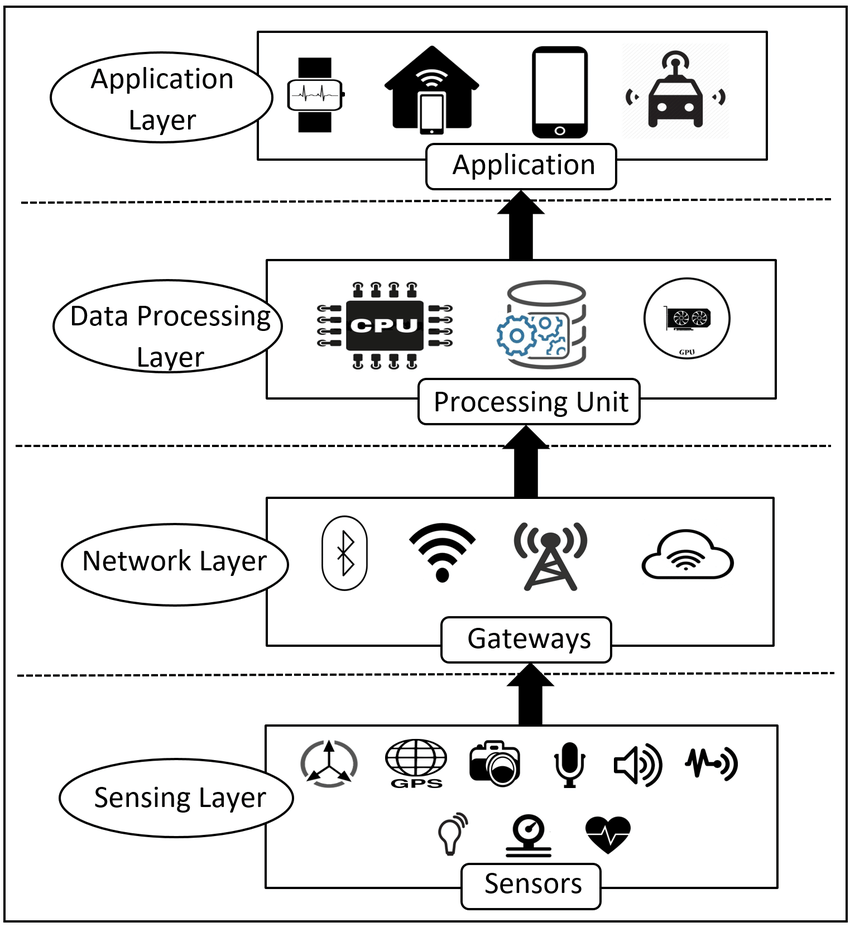
\includegraphics[width=0.7\linewidth]{figures/IoT-Architecture-Layers-and-Components.png}
%  \caption{Diagrama general de un sistema IoT}
%  \label{fig:IoT_General}
%\end{figure}


\section{Contexto tecnológico}

    En esta sección se describirán las tecnologías y herramientas más relevantes que se utilizarán a lo
    largo del desarrollo proyecto. El uso de las mismas se describirá en la sección \ref{chapter:desarrollo}.
    \todo[inline]{referenciar seccion correspondiente}
       
    \subsection{Android}

        A grandes rasgos, Android es un Sistema Operativo orientado a dispositivos móviles basado en el núcleo 
        Linux, diseñado para ser independiente de la arquitectura hardware de dichos dispositivos. 
        Si bien originalmente fue planteado para teléfonos móviles, con el avance de la industria ha adopado 
        un enfoque más amplio y es compatible con más dispositivos: tabletas, relojes inteligentes, televisores, 
        pantallas de automóviles, \textcolor{red}{etc.} %... 
        aunque, excepto en el caso de las tabletas, se trata de versiones basadas en
        Android con su propia %idionsincrasia
        \textcolor{red}{idiosincrasia}. 

        Normalmente cuando \textcolor{red}{se hace referencia a} %nos referimos a 
        Android \textcolor{red}{no se hace referencia} %, no nos referimos
        únicamente al sistema operativo, sino a la
        plataforma creada entorno al mismo; como \textcolor{red}{se hará} %haremos 
        a lo largo de este proyecto. Dicha plataforma o 
        \gls{framework} consta de numerosas capas, siendo el sistema operativo una parte de ellas. El sistema 
        operativo como tal es denominado AOSP o \textit{Android Open Source Project}, siendo su código fuente 
        público. Cualquier persona puede acceder a él, descargarlo y \textcolor{red}{modificarlo} %modificiarlo
        \cite{collado_que_2022}.

        \begin{figure}[h]
            \centering
            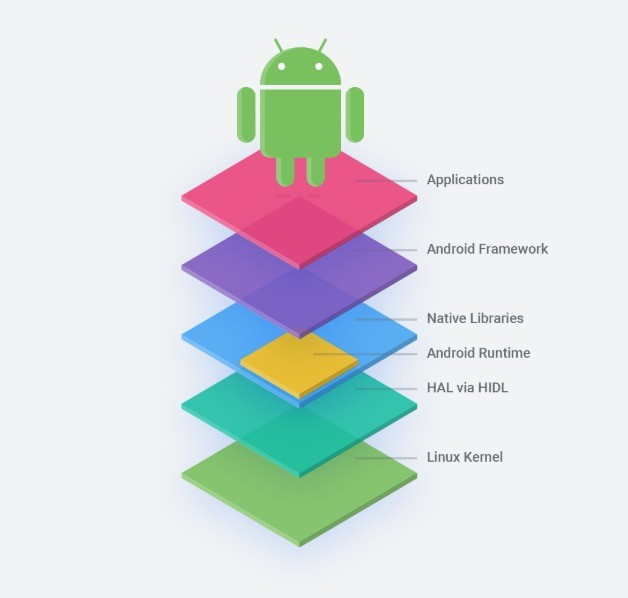
\includegraphics[width=0.66\textwidth]{figures/Android capas.jpg}
            \caption[Capas de Android.]
            {Capas de Android. Imagen extraída de \cite{perez_aosp_2019}}
            \label{figure:android:capas}
        \end{figure}

        No obstante, en la inmensa mayoría de los teléfonos móviles el sistema operativo es complementado con,
        entre otros, los GMS (\textit{Google Mobile Services}, o servicios de Google), los cuales solo están 
        disponibles bajo licencia; otorgada a los fabricantes que cumplen con una serie de requisitos. Los GMS 
        se utilizan para tareas como la gestión de notificaciones, servicios de geolocalización, ... además de para 
        acceder a las herramientas de Google, como la tienda de aplicaciones Play Store. Los fabricantes también 
        pueden personalizar y añadir funciones al sistema operativo, lo que explica que dos terminales con la misma 
        versión puedan verse tan diferentes entre sí. 
        

        Por otra parte, Android fue inicialmente desarrollado por la empresa homónima, si bien fue comprada en 2005
        por Google por 50 millones de dólares. La salida del sistema operativo se produciría dos años después, el 5 
        de noviembre de 2007, si bien el primer terminal que lo utilizaba (HTC Dream, también conocido como 
        T-Mobile G1) fue comercializado el 23 de septiembre de 2008 \cite{adeva_android_2023} \cite{marquez_asi_2022}.

        \begin{figure}[h]
            \centering
            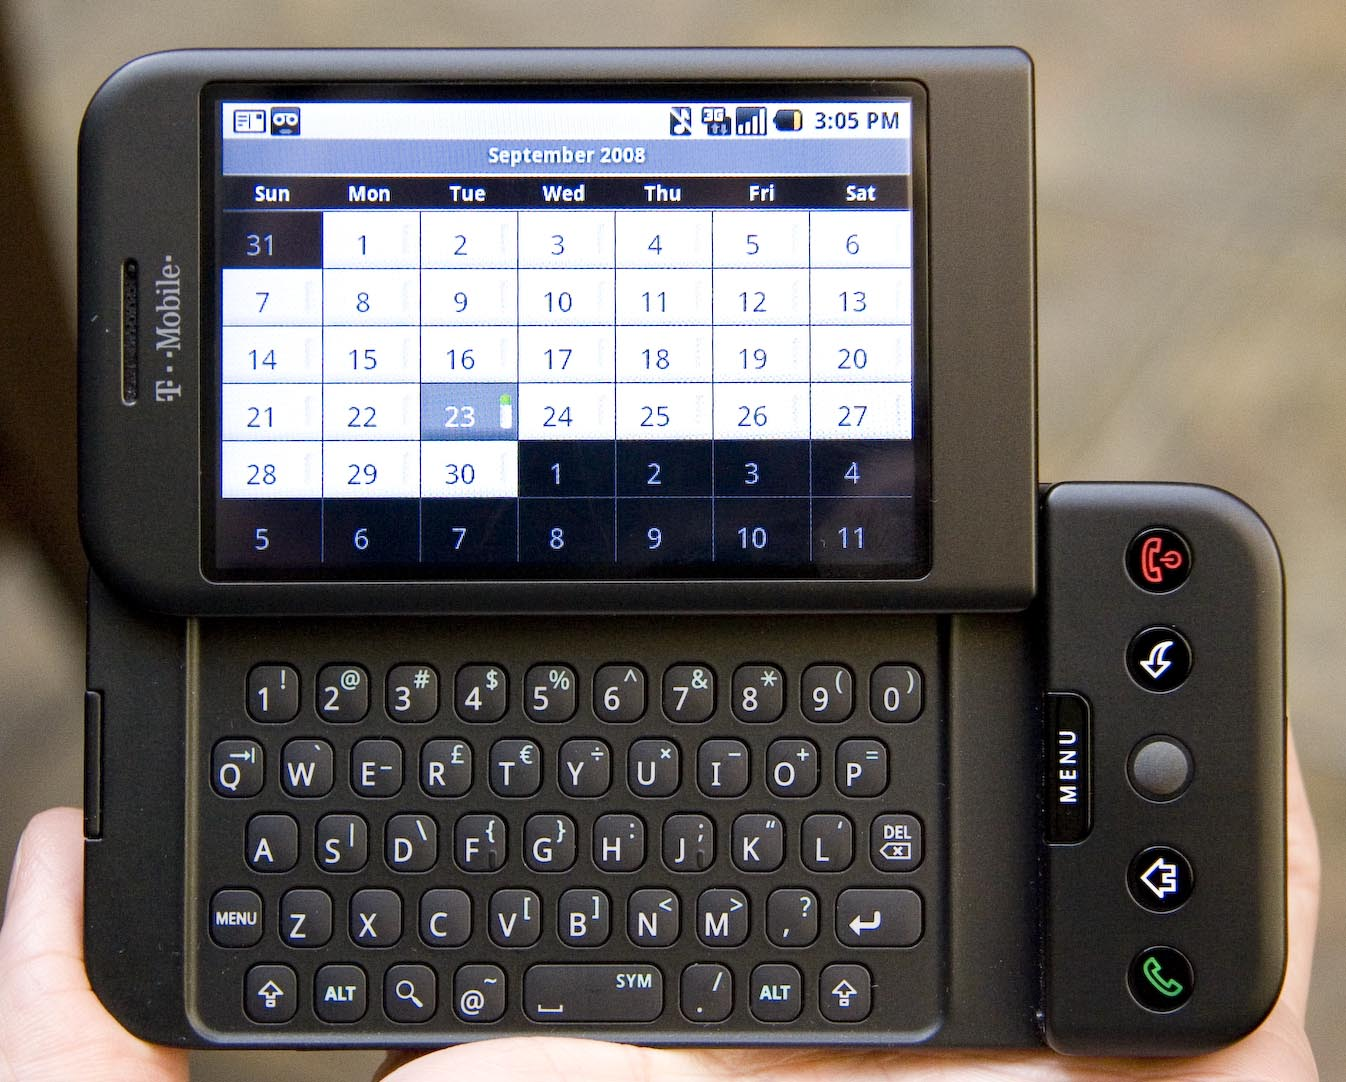
\includegraphics[width=0.5\textwidth]{figures/HTC Dream.jpg}
            \caption[HTC Dream en funcionamiento.]{HTC Dream en funcionamiento. Imagen extraída de \cite{oryl_t-mobile_2008}}
            \label{figure:android:htc_dream}
        \end{figure}

        Desde entonces, numerosas versiones de Android han sido lanzadas, siendo la última versión estable Android 
        13; estableciéndose por parte de Google la \textit{costumbre} de lanzar cada año una nueva versión principal. 
        En cada una de ellas se introducen nuevas características, pero esto no significa que todos los dispositivos 
        puedan actualizar. Los fabricantes no están obligados a actualizar sus terminales, lo que en la práctica 
        supone que las nuevas versiones no son utilizadas masivamente y que los programadores deben de tener en 
        cuenta las versiones antiguas en sus aplicaciones. 
        

        Debido a que Google dejó de publicar oficialmente las estadísticas de uso de su sistema operativo, no es
        posible conocer con plena exactitud dichas cifras. La comunidad se ha encargado de estimar dicha 
        información \cite{belinski_android_nodate}; relevando que a fecha de mayo de 2023 sólo el 20\% de los 
        dispositivos tienen la última versión, mientras que las versiones 12,11 y 10 están presentes en el 
        20,8\%, 21,1\% y 16,6\%, respectivamente. 

        \begin{figure}[H]
            \centering
            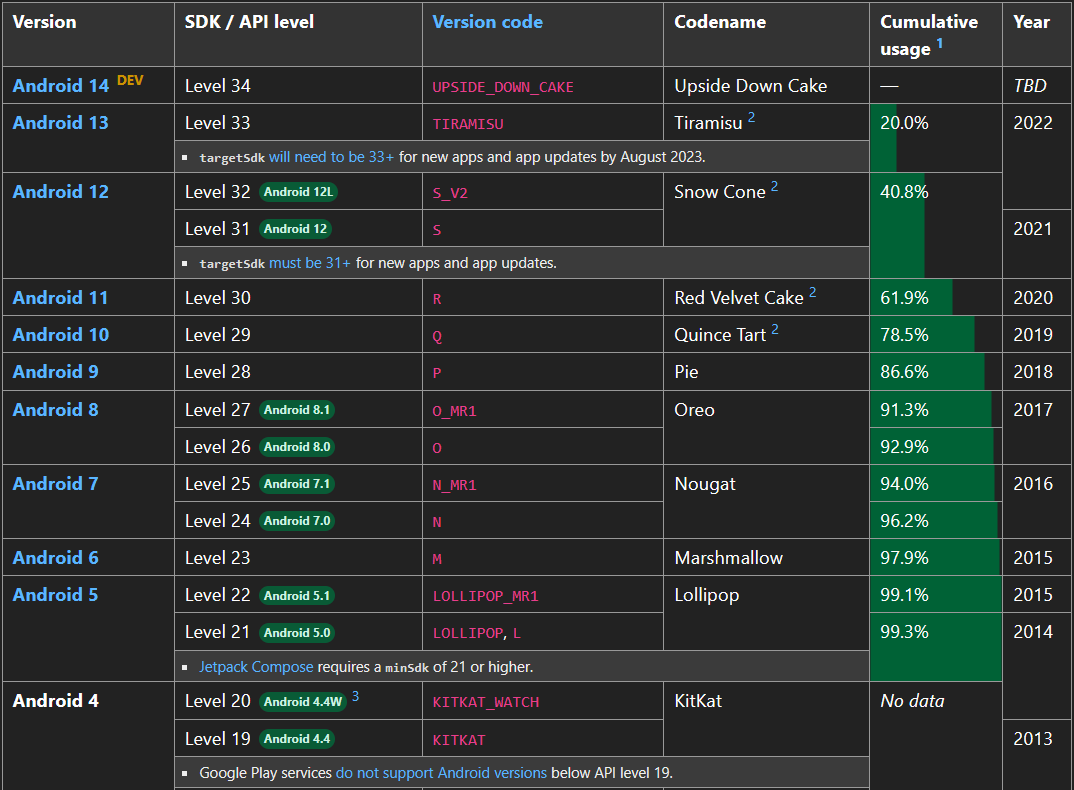
\includegraphics[width=1\textwidth]{figures/Android usage.PNG}
            \caption[Estadísiticas acumulativas de las versiones de Android]
            {Estadísiticas acumulativas de las versiones de Android. Imagen extraída de \cite{belinski_android_nodate}}
            \label{figure:android:usage}
        \end{figure}

        Por último, a fecha de marzo de 2023, Android dispone de una cuota de mercado del 71\% en el segmento de sistemas 
        operativos para dispositivos móviles, teniendo su mayor rival,el sistema operativo iOS (propiedad de Apple) 
        un 28\%. Entre ambos acaparan el mercado, con un 99\% de cuota de mercado. En cuanto a España, el 
        porcentaje de Android asciende hasta el 77,73\% por el 21,81 de iOS \cite{press_asi_2023}.

    \subsection{Kotlin}

            Durante el diseño de Android se estableció que el lenguaje principal para desarrollar aplicaciones sería 
            Java, si bien incorpora soporte para utilizar código C y C++ \cite{android_developers_como_nodate}. No
            obstante, al ser Java un lenguaje interpretrado sobre una máquina virtual (JVM o \textit{Java Virtual
            Machine}) se abrió la puerta para  utilizar otros lenguajes que utilizasen la JVM. En la conferencia de 
            Google \textit{I/O} de 2017 fue anunciado el soporte oficial y completo 
            de Kotlin dentro de Android. 

            Kotlin es un lenguaje de programación desarrollado por JetBrains\footnote{JetBrains es una
            empresa muy reconocida dentro de la industria por crear una serie de entornos de desarrollo muy populares,
            como PHPStorm, CLion o Intellij IDEA. Sobre este último está construido Android Studio, el entorno de 
            desarrollo oficial dentro de Android.} y publicada su primera versión estable el 15 de febrero de 2016.
            El objetivo de este lenguaje fue tan sencillo como ambicioso: crear un lenguaje conciso (permitiendo reducir
            la cantidad de código \textit{boilerplate}), con soporte de nuevas funcionalidades; pero sin renunciar a la rapidez de
            compilación de Java ni al todo el código escrito en él 
            \cite{rao_k_history_nodate}. 

            Sus principales características son las siguientes \cite{noauthor_kotlin_nodate} \cite{noauthor_enfoque_nodate}:
            \begin{itemize}
                \item Interoperable al 100\% con Java, lo que facilita la reutilización de código ya existentes. 
                Es interoperable en ambos sentidos.
                \item Permite escribir código más seguro, ya que en el diseño del lenguaje se solucionaron problemas
                crónicos de Java como las \textit{Null Pointer Exception}. Según datos internos de Google, las 
                aplicaciones escritas en Kotlin tienen un 20\% de probabilidades menos de fallar.
                \item Soporte nativo y estructurado para la programación concurrente y asíncrona mediante 
                construcciones como las corrutinas y los flujos.
                \item Desarrollo multiplataforma, no solo para Android: aplicaciones web, \textit{backend} e iOS.
                \item Permite desarrollos en varios paradigmas: orientada a objetos, funcional, imperativa...
            \end{itemize}
            
            Asimismo, al convertirse en la \textit{I/O} de 2019 en el lenguaje de referencia para el desarrollo 
            de Android \cite{braun_celebrating_2022}, los desarrollos de librerías y herramientas relacionadas con 
            Android están escritas en este lenguaje, aprovechando al máximo sus nuevas características. Por tanto, si
            bien es interoperable con Java, está recomendado que los nuevos desarrollos lo utilicen 
            \cite{lardinois_kotlin_2019}, como se ha realizado en este proyecto.
            
        \subsection{Jetpack Compose}

            Jetpack Compose es un conjunto de herramientas \textit{modernas} de Android para el desarrollo de 
            interfaces gráficas, lanzado en su primera versión estable el 28 de julio de 2021 por Google
            \cite{bellini_jetpack_2021}. Este kit de librerías permite desarrollar en el ecosistema Android de 
            forma nativa interfaces gráficas de manera declarativa como en los sistemas React, Flutter o SwiftUI;
            siguiendo las tendencias actuales de la industria en el desarrollo de aplicaciones móviles. 

            Este enfoque declarativo nos permite describir cómo queremos que sea nuestra interfaz gráfica. 
            Asimismo, las interfaces que construimos con este sistema pueden estar interconectadas a un estado 
            que definamos; describiendo cómo será nuestra interfaz para cada posible estado. Cuando ese estado cambie, 
            nuestra interfaz gráfica cambiará automáticamente para mostrar el nuevo estado, simplificando enormemente 
            el desarrollo y reduciendo el código necesario \cite{leiva_que_2021}. 

            Hasta la aparición de Jetpack Compose, el desarrollo interfaces gráficas nativas en Android se realizaba 
            con el enfoque conocido como programación imperativa. En este tipo de desarrollo es necesario especificar 
            paso por paso cómo se va a construir dicha interfaz gráfica exahustivamente. En dicho proceso (conocido 
            en Android como sistema de vistas) se codificaba un fichero XML, en el que se describían todos los 
            elementos gráficos (botones, textos...); para en el código Java/Kotlin de la aplicación se accediera 
            a dichos elementos y se le aplicaran manualmente modificaciones y transformaciones 
            \cite{noauthor_programacion_2021}. 

            Además, en Jetpack Compose, a diferencia del sistema anterior, los componentes gráficos están desacoplados 
            del sistema operativo; por lo que no dependemos de la versión del terminal para mostrar correctamente 
            nuestra interfaz gráfica. Eso ocurría anteriormente y como ya vimos, la fragmentación en Android es un 
            problema endémico, lo que complicaba bastante el desarrollo. Asimismo, es compatible con los componentes XML 
            del sistema anterior, lo que facilita la migración de los proyectos antiguos a este nuevo paradigma. 

            No obstante, como ya vimos en el apartado anterior, está diseñado para ser utilizado desde Kotlin, por lo 
            que en la práctica obliga a usar dicho lenguaje; lo que en algunos casos puede resultar en un pico de 
            dificultad hasta que se domina el lenguaje.

            Por último, esclarecer que Jetpack Compose es parte de un conjunto de librerías más grande conocido como 
            Android Jetpack, el cual es promovido por Google para mejorar el desarrollo dentro de Android 
            \cite{huaman_que_2018} \cite{noauthor_recursos_nodate}. Por otra
            parte, estas librerías no tienen ninguna relación entre sí; por lo que en la literatura especializada se 
            abusa de la notación. Al resto de las librerías de Jetpack se les conoce
            por su nombre, sin el prefijo Jetpack; siendo la única que lo incorpora Compose. En este documento 
            seguiremos ese enfoque para mejorar la legibilidad.
        
        \subsection{Material Design 3}
            Material Design 3 (también conocido como \textit{Material You}) es la tercera iteración del 
            conjunto de principios y directrices de diseño de Google, 
            como respuesta a la creciente ubiquidad de Android: móviles con pantallas
            plegables, \textit{smartwatch}, televisores \cite{ramirez_que_2022}... 
            Su primera implementación estable para Jetpack Compose fue lanzada el 
            24 de octubre de 2022 \cite{singh_material_2022}.
            
            Al ser utilizado por Google para la creación de elementos 
            gráficos tanto en sus aplicaciones como en el sistema operativo, es la guía de diseño de facto dentro del
            ecosistema Android.

            Sus principales características son las siguientes \cite{noauthor_material_nodate}:
            \begin{itemize}
                \item Centrado en la personalización de la interfaz gráfica. Los diseñadores definirán tres colores
                principales, los cuales serán utilizados para los elementos gráficos de forma totalmente transparente
                al programador. A partir de dichos colores, se elaborará mediante la herramienta 
                \textit{Material Design Builder} \cite{noauthor_material_nodate-1} una paleta de colores con 
                variantes de los mismos, 
                diseñada para cumplir estándares de accesibilidad\footnote{Describir dichos
                estándares está fuera del alcance del proyecto, pero es un proceso basado en proporciones de 
                luminitancia}, garantizando el nivel de contraste correcto.

                    \begin{figure}[h]
                        \centering
                        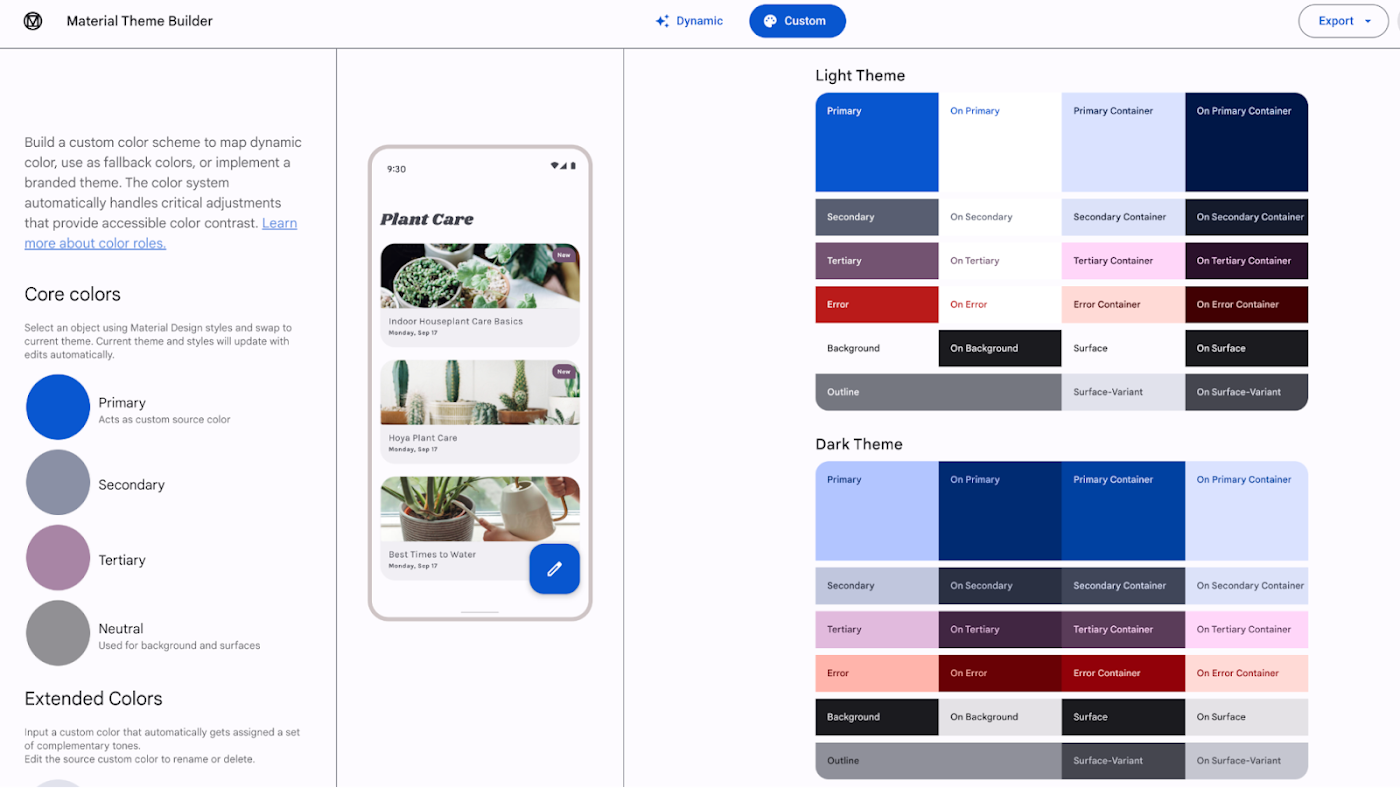
\includegraphics[width=0.75\textwidth]{figures/Material Design Builder example.png}
                        \caption[Ejemplo de uso de la herramienta \textit{Material Design Builder}]
                        {Ejemplo de uso de la herramienta \textit{Material Design Builder}. Imagen extraída de \cite{singh_material_2022}}
                        \label{figure:material_design_3:builder}
                    \end{figure}

                Además, si el dispositivo dispone de Android 12 o superior, pueden tomarse dichos
                colores desde el fondo de pantalla del usuario, incrementando exponencialmente la personalización;
                si bien se permite establecer colores \textit{fijos} para ciertos contenidos.
                \item Soporte nativo para categorizar el tamaño de la pantalla del dispositivo, tanto en altura como
                en anchura.
                    \begin{figure}[h]
                        \centering
                        \includegraphics[width=0.75\textwidth]{figures/Tamaños de ventana.png}
                        \caption[Categorías de pantalla según anchura]
                        {Categorías de pantalla según anchura. Imagen extraída de \cite{singh_material_2022}}
                        \label{figure:material_design_3:width_classes}
                    \end{figure}
                \item Sistema de fuentes basado en estilos principales para cada tipo de contenido: desde titulares 
                hasta etiquetas, pasando por títulos, cuerpos de texto...
                \item Soporte nativo para animaciones, las cuales ya son utilizadas en los componentes gráficos nativos,
                como los \textit{switch}.
                \item Evolución de muchos elementos gráficos, como las tarjetas, botones, selectores de fechas...
                    \begin{figure}[h]
                        \centering
                        \includegraphics[width=0.75\textwidth]{figures/Elementos gráficos material design 3.png}
                        \caption[Algunos elementos gráficos de Material Design 3]
                        {Algunos elementos gráficos de Material Design 3. Imagen extraída de \cite{cerda_material_2022}}
                        \label{figure:material_design_3:elementos_graficos}
                    \end{figure}
                \item Sistema de formas o \textit{redondeo} multinivel para modernizar nuestros elementos y hacerlos
                más distingubles entre sí.
        
                \item Mejora el concepto conocido como \textit{elevación}, basándose en colores y no en sombras. Este
                elemento permite superponer elementos y transmitir gráfica y visualmente la importancia de cada 
                uno de ellos.
                \item Soporte nativo para tema claro y oscuro, ya que en los últimos años los temas oscuros 
                se han hecho cada vez más populares en las aplicaciones y no estaba presente previamente de forma nativa.
            \end{itemize}

            En pocas palabras, en esta versión se han dedicado a modernizar el lenguaje de diseño, haciéndolo más 
            atractivo y completo; alejándose de lo puramente funcional, mejorando la accesibilidad y explorando 
            el mundo de la personalización para el usuario.

        \subsection{Salud Conectada}
            \label{section:salud_conectada}
            En la conferencia \textit{I/O} (sí, otra vez) de 2022 se anunció \textit{Health Connect} (o Salud Conectada
            en castellano), una aplicación creada por Google (junto con Samsung \cite{wilk_introducing_2022}) 
            que aglutinará todos los datos relacionados con salud dentro del ecosistema
            Android. La aplicación (en beta desde noviembre de 2022) es compatible con Android 9 o 
            superior, mientras que está previsto que para Android 14 venga
            incorporada aplicación de fábrica o preinstalada\footnote{Recordar aquí que esta aplicación es
            parte de los servicios de Google y no del sistema operativo propiamente dicho o AOSP.} 
            \cite{pandey_health_2023}. 

            Esta herramienta viene a solucionar una probelmática importante y es la ausencia del reaprovechamiento de 
            los datos relacionados con la salud. Hasta ese momento, la posición casi unánime dentro la 
            industria se basaba en aislar los datos recoletados por sus dispositivos \textit{\glspl{wearable}} o aplicación 
            dentro de su ecosistema \cite{ramirez_android_2022} \cite{rahman_android_2023}. 
            
            La única manera utilizar dichos datos 
            en otras aplicaciones estaba restringuida a sistemas propietarios como Google Fit, cuyos datos se 
            almacenaban enla nube con los problemas de privacidad asociados, o proyectos \textit{open source} como 
            Gadget Bridge \cite{freeyourgadget_gadgetbridge_nodate}; que accedían a datos mediante ingeniería inversa.
            

            A fecha de mayo de 2023, se estima que más de 100 aplicaciones han integrado Salud Conectada, incluyendo
            las aplicaciones de las pulseras Fitbit y Samsung, Peloton, Oura \cite{malik_googles_2023}... 

            Centrándonos en Salud Conectada, se trata tanto de una plataforma como una API para los desarrolladores.
            La plataforma puede registrar datos como la actividad física, el sueño, la nutrición o incluso el ciclo
            menstrual\footnote{La lista completa de los datos que puede registrar Salud Conectada se encuentra 
            disponible en \cite{noauthor_lista_nodate}}, siendo un intermediario entre las aplicaciones que generan 
            o escriben dichos datos y las que quieren acceder a esos datos. 

            \begin{figure}[h]
                \centering
                \includegraphics[width=0.33\textwidth]{figures/Arquitectura básica de Health Connect.png}
                \caption[Arquitectura básica de Salud Conectada.]
                {Arquitectura básica de  Salud Conectada. Imagen extraída de \cite{wilk_introducing_2022}}
                \label{figure:health_connect:arquitectura}
            \end{figure}

            Esta API estandariza el acceso a todas las fuentes de datos, independientemente de su procedencia; lo que
            simplifica enormemente tanto la lectura como escritura de los datos. Además, el sistema permite consultar
            datos agregados, pudiendo ser una agregación acumulativa (como el total de distancia caminada en un 
            intervalo de tiempo) o estadística (las pulsaciones mínimas, máximas o promedio en un intervalo de tiempo).

            \begin{figure}[h]
                \centering
                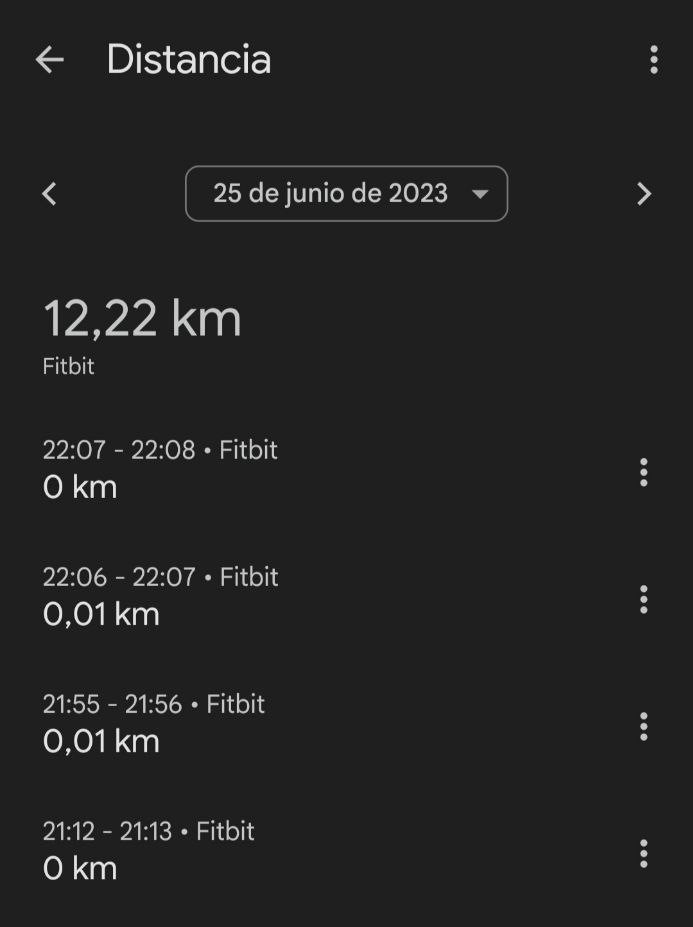
\includegraphics[width=0.33\textwidth]{figures/Health Connect lectura datos.jpg}
                \caption[Visualización de datos de distancia.]
                {Visualización de datos de distancia.}
                \label{figure:health_connect:visualizacion_datos}
            \end{figure}
            
            Por otra parte, está diseñada con la privacidad en mente: los datos se almacenan localmente, mientras que el 
            acceso a los mismos esta fuertemente granularizado: en la que el usuario puede
            decidir qué aplicaciones tienen acceso (tanto lectura como escritura) a cada tipo de registro 
            \cite{saez_google_2022}.  
            
            \begin{figure}[h]
                \centering
                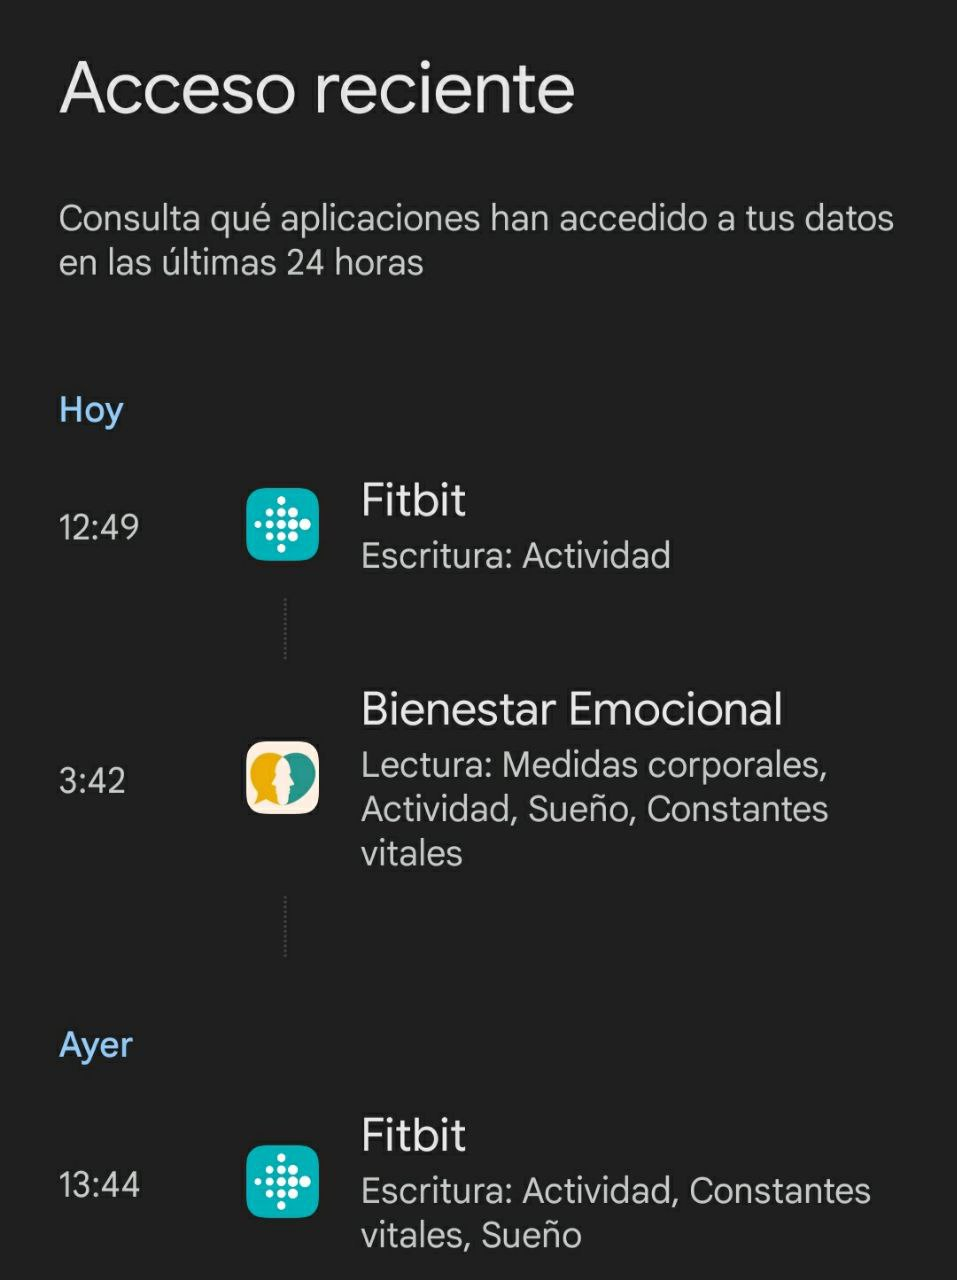
\includegraphics[width=0.33\textwidth]{figures/Health Connect acceso reciente.jpg}
                \caption[Visualización del acceso a los datos.]
                {Visualización del acceso a los datos. Elaboración propia.}
                \label{figure:health_connect:acceso_reciente}
            \end{figure}

            
            Asimismo, las aplicaciones solo pueden leer datos con una antigüedad de 
            hasta 30 días previos a su instalación. \cite{noauthor_preguntas_nodate}, registrándose además todas las 
            lecturas y escrituras en el sistema, las cuales puede visualizar el usuario. 

            \begin{figure}[h]
                \centering
                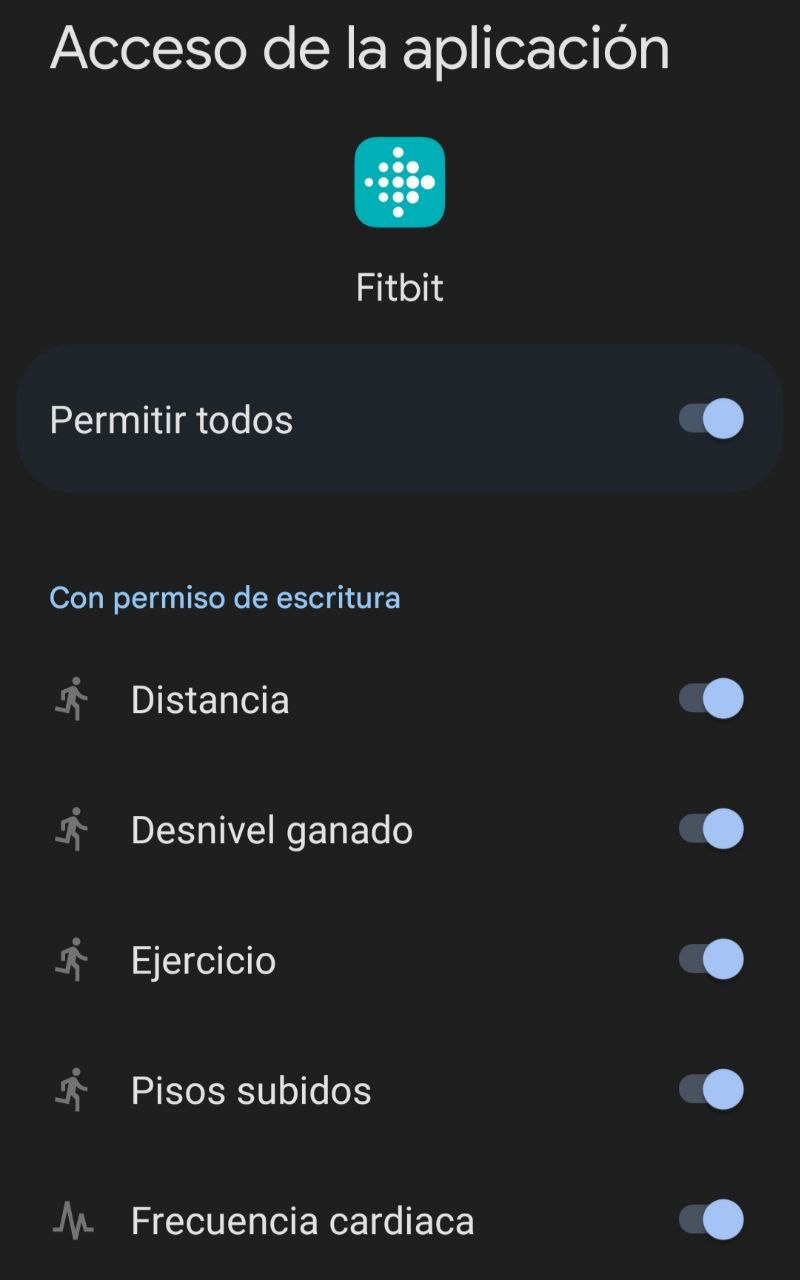
\includegraphics[width=0.33\textwidth]{figures/Health connect permisos fitbit.jpg}
                \caption[Granularidad de los permisos.]
                {Granularidad de los permisos. Elaboración propia.}
                \label{figure:health_connect:granularidad_permisos}
            \end{figure}

            En definitiva, si bien está aún en desarrollo, esta plataforma nos permite abstraernos del hardware de
            recolección de datos biométricos, reduciendo la complejidad de nuestro desarrollo; y además permite al 
            usuario un mayor control sobre sus datos sensibles.
            
        \subsection{Room}
            Uno de los servicios que provee Android es SQLite, un sistema de gestión de base de datos relacionales de 
            bajo nivel. Este sistema es usado por la aplicación que lo utiliza, ahorrando configuración y complejidad
            \cite{recio_persistencia_2019}. 
            
            No obstante para muchas aplicaciones es un modelo demasiado rígido. Para simplificar el uso de SQLite
            Google creó en 2017 esta librería, la cual hace de intermediario entre el propio SQLite y nuestra 
            aplicación \cite{leiva_room_2020}. Técnicamente hablando se trata de una capa de abstracción sobre dicho
            sistema gestor, la cual permite reducir la complejidad de los usos comunes de la base de datos; sin perder
            el acceso a SQLite. Asimismo, esta librería brinda otras ventajas, como la verificación de las consultas
            SQL en tiempo de compilación \cite{noauthor_como_nodate}.

            Los elementos básicos de esta plataforma son los siguientes:
            \begin{itemize}
                \item \textit{Data Access Objects}, también conocido como DAO. En este elemento (implementado como
                una interfaz con la anotación @Dao) creamos nuestras
                operaciones sobre la base de datos: consultas, inserciones...
                \item Entidades, las cuales se corresponden con una clase en Kotlin (anotada como @Entity)
                y normalmente con una tabla de base de datos.
                Con esta estructura creamos las tablas de la base de datos, mientras que en nuestra aplicación 
                disponemos de objetos que mapean dichos registros. Los atributos de dicha clase serán los campos de
                la tabla en cuestión, sobre los cuales podemos utilizar anotaciones para establecer claves, índices, etc
                \item Clase base de datos, donde especificamos las entidades a utilizar y cómo se instancia dicha base
                de datos (aquí podemos ajustar si estará cifrada o no por ejemplo). Se corresponde con una clase 
                abstracta que hereda de \textit{RoomDatabase} y que usa ciertas anotaciones para que se genere 
                automáticamente el código \textit{boilerplate}.
                \item Una función que construya la instancia de dicha base de datos con la configuración deseada
                (nombre del fichero de la base de datos, cifrado..). Para dicha construcción de la instancia Room
                implementa el patrón factoría.
            \end{itemize}
            
        \subsection{Dagger Hilt}
            Dagger Hilt es una biblioteca que permite la automatización de la inyección de dependencias dentro de 
            nuestra aplicación; la cual es la opción promovida por Google para esta tarea. El nombre
            compuesto no es casual, ya que hace referencia a que en realidad son dos librerías: Dagger realiza el
            trabajo de la inyección de dependencias, mientras que Hilt es la integración estándar de Dagger en Android 
            \cite{noauthor_insercion_nodate}, simplificando el proceso y facilitando la curva de aprendizaje de Dagger
            \cite{leiva_dagger_2020}.

            Para poder utilizar esta librería, es obligatorio marcar un punto de arranque en la aplicación para que se
            inicialice el sistema de dependencias. Asimismo, se debe indicar que Dagger Hilt debe inyectar dependencias 
            en cada caso que corresponda. Por otra parte, se necesitan definir uno o más módulos, en los 
            cuales se indica a Dagger Hilt cómo construir las dependencias, el alcance de las mismas y otras
            características. 
            
            Esto nos permite que algunas dependencias sean construidas con una única instancia para
            todo el proyecto, mientras que otras puedan ser instanciadas en múltiples ocasiones, o con un ciclo de vida 
            asociado al de algunos componentes de Android (como los ViewModel).

            En resumen se trata de una tecnología auxiliar que nos permite realizar una inyección de dependencias
            eficaz sin demasiada complejidad de uso.

        \subsection{Work Manager}
            Work Manager es el componente oficial de Android para la planificación de subtareas dentro de nuestra 
            aplicación. Esta librería está diseñada para simplificar el uso del amalgama de librerías para esta
            funcionalidad, ya que, según la versión del sistema, debían utilizarse unas u otras. Work Manager establece
            una única interfaz para esta funcionalidad, encargándose internamente de utilizar la librería correcta a
            bajo nivel \cite{noauthor_workmanager_nodate}.
            
            Este componente admite dos tipos de tareas: puntuales y periódicas; las cuales se pueden planificar o 
            cancelar. Asimismo, además de la planificación temporal, permite el establecimiento de algunas restricciones,
            como que el dispositivo esté cargándose o disponga de conexión a internet, ejecutándose la tarea en cuestión
            cuando se cumplan al mismo las directrices temporales y las adicionales (si las hay) 
            \cite{noauthor_arquitectura_nodate}.

            Asimismo, nos permite establecer una política de reintentos si nuestras tareas no se ejecutan correctamente,
            por lo que es la solución recomendada para cuando necesitamos realizar cierta funcionalidad de manera fiable.
            
            \todo[inline]{Los problemas que da los comentamos de pasada referenciando a stackoverflow o ya al final?
            Por mi solo al final.}

        \subsection{Retrofit}
            Retrofit es una librería muy popular en el ecosistema Android, ya que nos proporciona una capa de alto nivel
            para el consumo de API. En particular, nos permite interactuar con dichos recursos de una manera estructurada
            y orientado a objetos (o a entidades). Además proporciona soporte nativo para el uso de corrutinas, por lo
            que nos permite realizar llamadas remotas de forma concurrente, sin bloquear el hilo principal de nuestra
            aplicación.

            Esta biblioteca trabaja junto con otros componentes software conocidos como serializadores, los cuales se 
            encargan de convertir nuestros objetos Kotlin a formato json, los cuales son necesarios para interactuar
            con los recursos en red. Retrofit soporta una lista de ellos, pero en este proyecto utilizaremos el 
            incorporado por defecto: gson, creado y mantenido por Google.

            Sus elementos básicos son los siguientes \cite{noauthor_retrofit_nodate} \footnote{Es posible que te 
            recuerde a los componentes de Room y 
            no es casualidad, ya que ambas están diseñadas de una manera similar, utilizando los mismos patrones de
            diseño software}:
            \begin{itemize}
                \item Entidades, las cuales mapean el formato json necesario (ya sea para enviar o recibir datos) con 
                una clase en Kotlin.
                \item Una interfaz donde se asocian las llamadas a la API (ruta y tipo) que utilizaremos junto a la 
                cabecera de la función que implementará Retrofit automáticamente. Aquí le indicaremos, si procede, los
                parámetros de la llamada y el resultado de la misma, los cuales serán normalmente entidades que habremos
                definido previamente.
                \item Una función que construya una instancia de la interfaz anterior, donde se le indica la url base de
                la API en cuestión y configuración adicional, como el serializador a utilizar.
            \end{itemize}
            
        \subsection{Lottie}
            Lottie es una biblioteca creada por Airbnb que busca facilitar la creación y uso de animaciones en entornos
            multiplataforma (web, iOS, Android..) \cite{rubianes_lottie_2021}. A diferencia de archivos como los GIF, 
            esta librería permite que
            las animaciones puedan escalarse sin perder calidad (como en los ficheros SVG), haciendo hincapié en el
            rendimiento.

            Concretamente, la librería renderiza en tiempo real animaciones de Adobe After Effects, las cuales
            son exportadas como ficheros JSON que serializan dicha animación \cite{noauthor_lottie_nodate}, a través de
            una extensión de código abierto conocida como Bodymovin. Por tanto, 
            estas animaciones pueden
            ser personalizadas completamente, a la vez que se reducen las necesidades de cómputo para mostrarlas. 
            
            \begin{figure}[h]
                \centering
                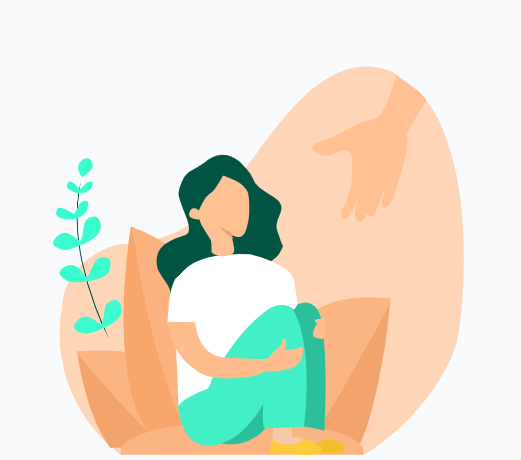
\includegraphics[width=0.33\textwidth]{figures/Animacion de ejemplo.PNG}
                \caption{Vista previa de una animación personalizada}
                \label{figure:lottie:animacion_ejemplo}
            \end{figure}

            En este proyecto abordaremos únicamente la personalización de animaciones gratuitas aportadas por la 
            comunidad y su presentación en la aplicación; y no la creación de nuevas. Para conseguir dichas animaciones
            se ha utilizado el portal \href{https://lottiefiles.com/}{LottieFiles}.

        \subsection{Vico}
            
            Vico es una biblioteca open-source para la realización de gráficos, creada pòr Patryk Goworowski. Su 
            particularidad reside en su compatibilidad tanto con el sistema de vistas tradicional como con Jetpack
            Compose, algo único en el ecosistema de Android \cite{goworowski_vico_nodate}.

            Si bien no es tan potente como otras librerías como \textit{MPAndroid}, sus posibilidades son más que 
            suficientes para este proyecto, aligerando el desarrollo. Además su soporte nativo de Jetpack
            Compose reduce la complejidad del desarrollo e introduce algunas mejoras, como una interconexión
            directa con los colores que usará Jetpack Compose para los elementos gráficos, mejorando la calidad visual
            de la aplicación.

            \begin{figure}[h]
                \centering
                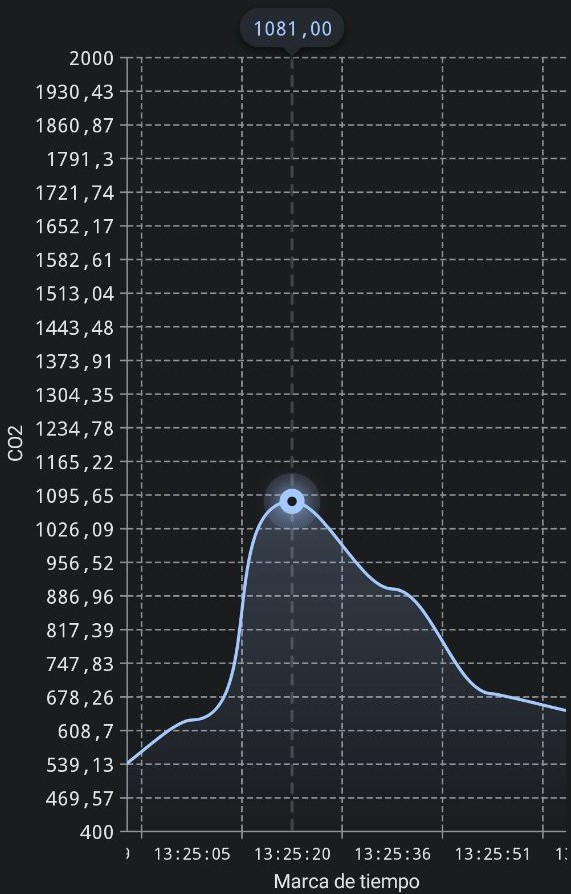
\includegraphics[width=0.33\textwidth]{figures/Gráfica de líneas con vico.jpg}
                \caption{Ejemplo de gráfica de líneas con Vico}
                \label{figure:vico:ejemplo_lineas}
            \end{figure}

            Vico nos permite crear únicamente gráficos de barras y de líneas. Su humilde enfoque, si bien puede
            condicionar su uso, permite que contenga numerosos añadidos completamente personalizables, tales como
            leyendas, marcadores (tanto fijos como temporales), \textit{líneas umbral}, personalización programática 
            de los ejes...

            \begin{figure}[h]
                \centering
                \includegraphics[width=0.5\textwidth]{figures/Gráfica de barras con vico.jpg}
                \caption{Ejemplo de gráfica de barras con Vico}
                \label{figure:vico:ejemplo_barras}
            \end{figure}
            
            Asimismo, su mantenimiento y mejora es notable y constante. Nuevas versiones son lanzadas
            cada pocas semanas \cite{goworowski_vico_2023-1}, mientras que el soporte ofrecido en su repositorio 
            es rápido y detallado \cite{goworowski_vico_2023}. Además, dispone de numerosa documentación para
            aprenderla rápidamente, si bien no cubre los casos de uso más avanzados.

            Por último, dispone de una aplicación demo que permite ver rápidamente las posibilidades que ofrece la 
            librería.
    
        \subsection{Python}
            Python es un lenguaje de programación interpretado creado por Guido Van Rossum en 1991, con un marcado enfoque 
            de construir código de la manera más clara y legible posible. Es uno de los lenguajes más populares de la 
            escena, gracias a su facilidad de uso y a su enorme comunidad de desarrolladores. Estos últimos han creado un 
            enorme ecosistema de librerías que facilita la creación de nuevos proyectos, especialmente para prototipos.

            Actualmente es utilizado para todo tipo de tareas, tales como desarrollo web, aplicaciones científicas… 
            pasando por inteligencia artificial o análisis de datos; casi siempre apoyándose en potentes librerías 
            que mejoran notablemente el propio lenguaje. 

            Sus principales características son las siguientes:
            \begin{itemize}
                \item Soporte mutiparadigma: como Kotlin, se puede utilizar programación imperativa, orientada a objetos o 
                funcional en cualquier momento.
                \item Gran biblioteca estándar que facilita muchas operaciones mundanas, como la lectura de archivos JSON.
                \item Soporte multiplataforma gracias a la compatibilidad de su intérprete con todos los sistemas 
                operativos principales. Llega hasta tal punto que un subconjunto del lenguaje (MicroPython) es compatible 
                con algunos microcontroladores.
                \item Sistema de tipos fuertemente tipado y dinámico, lo que permite que una variable pueda cambiar de 
                tipo fácilmente.
                \item Facilidad de instalación de librerías gracias a la herramienta pip.
            \end{itemize}
        
        \subsection{Flask}

            Flask es un popular entorno ligero o \textit{microframework} de Python utilizado para construir aplicaciones 
            web, tanto como páginas como API. Diseñado para ser ligero y fácil de usar, Flask proporciona las herramientas 
            necesarias para crear dichas aplicaciones web de una manera minimalista, rápida y eficiente, en sintonía con 
            la propia filosofía del lenguaje. 

            A diferencia de otros entornos más completos como Django, Flask se enfoca en brindar solo lo esencial, lo que 
            permite crear prototipos lo más fácilmente posible, si bien puede quedarse corto para aplicaciones 
            relativamente complejas \cite{rodriguez_flask_2014}. Su sistema de enrutamento HTTP es sencillo y claro, mientras que posee extensiones 
            para autentificación de usuarios, manejo de base de datos, etc. 

            Gracias a esta simplicidad se usará en este proyecto para prototipar la parte del servidor. Asimismo, debido a 
            su enfoque modular y a su sistema de plantillas podría expandirse su funcionalidad con más elementos web sin 
            ninguna adaptación del código ya existente.


        \subsection{MongoDB}
            MongoDB es un sistema gestor de base de datos no relacional orientado a documentos, diseñado para manejar 
            grandes volúmenes de datos de manera eficiente y escalable. A diferencia de las bases de datos relacionales 
            tradicionales, no hay registros sino documentos, unos ficheros con una extensión muy similar a JSON: BSON 
            (JSON Binarios) \cite{noauthor_json_nodate}. 

            Este enfoque no relacional le permite ofrecer un modelo de datos flexible, sin un esquema. Esto se traduce
            en una mayor libertad para almacenar datos y cambiar el modelo de los mismos, ya que para cambiar cualquier
            atributo no es necesario reconstruir el modelo; muy útil para prototipos o modelos de datos dinámicos.
            

            Por otra parte, el modelo de consultas ofrece posibilidades similares a las de SQL, por lo que no supone
            una desventaja. También implementa conceptos presentes en las base de datos relacionales, como los índices. 
            Además, al disponer de una gran comunidad detrás, existen numerosos módulos que lo permiten
            intregrar con lenguajes de programación, como pymongo para Python. 

            Asimismo, posee otras dos grandes fortalezas: un núcleo distribuido, lo que permite una alta disponibilidad
            y escalabilidad; y una licencia de uso gratuito desde octubre de 2018, bajo la licencia AGPL 
            \cite{noauthor_que_nodate}.
    \subsection{Git, GitHub y GitHub Actions}
        Git es un extremadamente popular y utilizado sistema de control de versiones distribuido libre y gratuito,
        creado por Linus Torvalds, creador de Linux. Es utilizado para guardar diferentes versiones
        de un conjunto de archivos, conocido como repositorio; pudiéndose recuperar en cualquier momento
        cualquier versión del mismo, a la vez que se guarda un registro de cuándo, quién y qué cambios se han 
        realizado entre versiones \cite{atlassian_software_nodate}.

        Asimismo, Git, como otros sistemas de control de versiones, dispone de herramientas para la integración de
        cambios de varios usuarios, algo muy útil en el desarollo de software. Por otra parte, al ser distribuido,
        se dispone una copia de todo el repositorio en cada máquina, por lo que no dependemos de un nodo central
        para poder trabajar; si bien se define normalmente un nodo remoto que hace las veces de \textit{punto de
        encuentro} entre los distintos nodos. 

        Por otra parte, GitHub es una plataforma web, propiedad de Microsoft, donde los usuarios pueden alojar
        repositorios Git tanto públicos como privados; facilitando los procesos de compartir código y de 
        colaboración en proyectos de otros programadores. GitHub no es la única plataforma para este proceso: Gitlab
        y Bitbucket son algunas de las alternativas \cite{noauthor_git_2021}. 

        El potencial de GitHub no acaba ahí: gracias a su extensión Acciones (o Actions en inglés) permite que en
        los repositorio se puedan automatizar y ejecutar flujos de trabajo, lo que abre las puertas a la ejecución
        de flujos de integración y despliegue (o entrega) continuo, conocidos como CI/CD.

        En este proyecto se ha elegido Git para la gestión del código software como el del presente documento,
        mientras que el uso de GitHub se debe tanto para almancenar una copia de seguridad del código adicional, 
        para la mejora de la visibilidad del proyecto y por último para poder configurar y ejecutar flujos de CI/CD
        para nuestro software.